\begin{frame}{第二十六讲、定积分的应用}
	\linespread{1.5}
	\begin{enumerate}
	  \item {\bf 内容与要求}{\b( \S 6.4 )}
	  \begin{itemize}
	    \item 掌握用定积分求解应用问题的基本方法
	    \item 了解如何用定积分求解几何问题
	    \item 了解如何用定积分求解物理问题
	  \vspace{1em}
	  \end{itemize}
	  \item {\bf 课后作业:}
	  \begin{itemize}
 	    \item 书面作业:
	     {\b 习题6.4:2,5,6(1),8,10,11,15,16,19}
% 	    \item {\b 习题6.3:8,9,12,14,18}
  	    \item 思考题:{\b 习题6.4:1-30其余各题}
	  \end{itemize}
	\end{enumerate}
\end{frame}

\begin{frame}{定积分的构造思路──微元法}
	\linespread{1.2}
	\begin{columns}
		\column{.5\textwidth}
		\begin{enumerate}
		  \item {\bb 分割:}沿$x$轴方向分割曲边梯形\pause 
		  \item {\bb 取近似:}用小矩形的面积$\Delta S$近似小曲边梯形面积\pause 
		  \item {\bb 做和:}求所有小矩形的面积总和$\sum \Delta S$\pause 
		  \item {\bb 求极限:}$\sum \Delta S\to S$
		\end{enumerate}
		\column{.55\textwidth}
		\begin{center}
			\resizebox{!}{5.5cm}{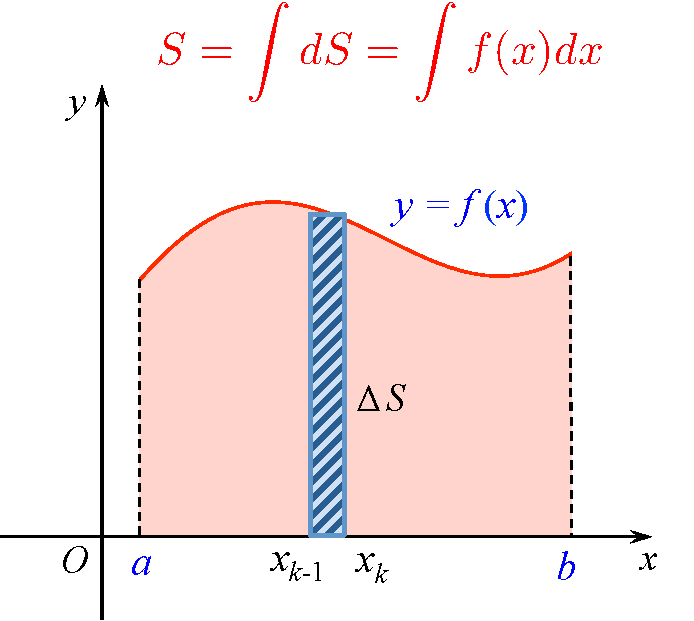
\includegraphics{./images/ch6/sumSSS.pdf}}
		\end{center}
	\end{columns}
\end{frame}

\section{用定积分求解几何问题}

\begin{frame}{平面直角坐标系情形}
	\linespread{1.2}\pause 
	\begin{exampleblock}{{\bf 例1}\hfill}
		计算两条抛物线$y^2=x$和$y=x^2$所谓图形的面积。
	\end{exampleblock}
	\vspace{2em}
	\pause 
	\begin{exampleblock}{{\bf 例2}\hfill}
		计算两条抛物线$y^2=2x$与直线$y=x-4$所谓图形的面积。
	\end{exampleblock}
\end{frame}

\begin{frame}{极坐标情形}
	\linespread{1.2}\pause 
	\begin{exampleblock}{{\bf 例3}\hfill}
		计算Archimedes螺线
		$\rho=a\theta\;(a>0)$
		相应于$\theta$从$0$变到$2\pi$的一段弧与极轴所围的图形面积。
	\end{exampleblock}\pause 
	\begin{center}
		\resizebox{!}{4cm}{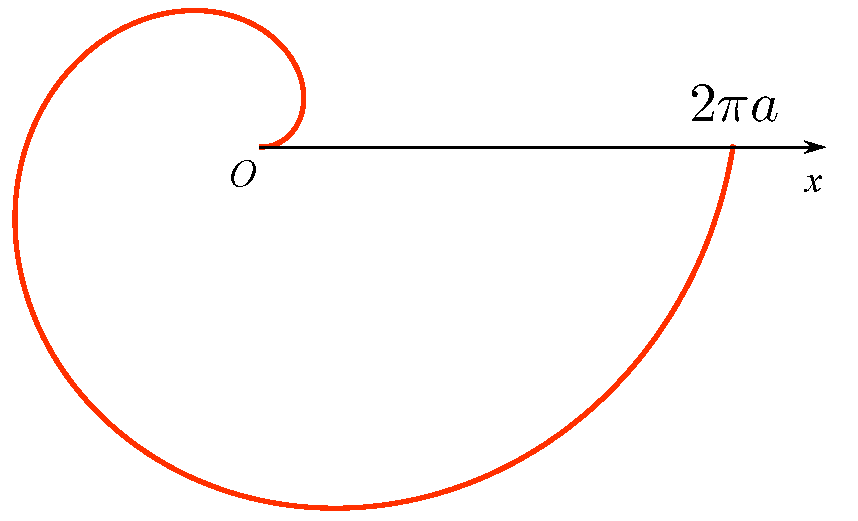
\includegraphics{./images/ch6/Achimedes.pdf}}
	\end{center}
\end{frame}

\begin{frame}{旋转体的体积}
	\linespread{1.8}\pause 
% 	\begin{exampleblock}{{\bf 例4}\hfill}
% 		连接坐标原点$O$及点$P(h,r)$的直线、直线$x=h$与$x$轴共同围成一个直角三角形,
% 		求该三角形绕$x$轴旋转一周所得立体的体积。
% 	\end{exampleblock}
	{\bb 曲线$y=f(x)\;(x\in[a,b])$绕$x$轴旋转一周:}\pause
	$$\alert{V=\dint_a^b\pi[f(x)]^2\d x}$$
	\pause
% 	\bigskip
% 	\vspace{1em}
	\begin{exampleblock}{{\bf 例4}\hfill}
		求椭圆$\df{x^a}{a^2}+\df{y^2}{b^2}=1$绕$x$轴旋转一周所得立体的体积。
	\end{exampleblock}
\end{frame}

\begin{frame}
	\linespread{1.2}
	\begin{exampleblock}{{\bf 例5}\hfill}
		计算由圆滚线$$x=a(t-\sin t),y=a(1-\cos t)\;(0\leq t\leq 2\pi)$$
		和直线$y=0$所围图形分别绕$x$轴、$y$轴旋转一周所得立体的体积。
	\end{exampleblock}
\end{frame}

\begin{frame}{已知截面积的立体体积}
	\linespread{1.2}
	\begin{exampleblock}{{\bf 例6}\hfill}
		一平面经过半径为$R$的圆柱体的底面圆心,并与底面交角为$\alpha$(如图所示),求该平面所截圆柱体
		的体积。
	\end{exampleblock}\pause 
	\begin{center}
		\resizebox{!}{4.5cm}{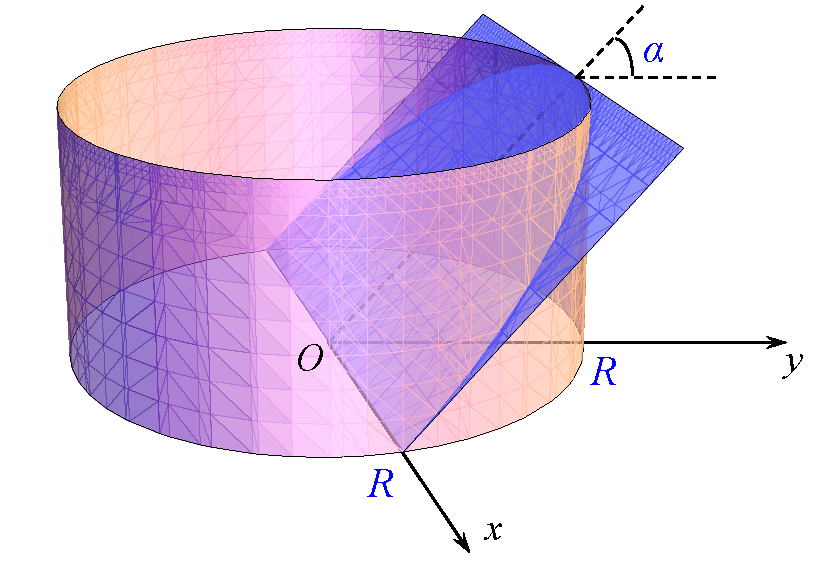
\includegraphics{./images/ch6/bucket.pdf}}
	\end{center}
\end{frame}

\begin{frame}{平面曲线的弧长}
	\linespread{2}
	\begin{exampleblock}{{\bf 例7:}求以下曲线的弧长\hfill}\pause 
		\begin{enumerate}
		  \item $y=\df 23x^{3/2}\;(a\leq x\leq b)$\pause 
		  \item $x=a(t-\sin t),y=a(1-\cos t)\;(0\leq t\leq 2\pi)$\pause 
		  \item $\rho=a\theta\;(a>0,\;0\leq t\leq 2\pi)$
		\end{enumerate}
	\end{exampleblock}
\end{frame}

\section{用定积分求解物理问题}

\begin{frame}{变力沿直线做功}
	\linespread{1.2}
	\begin{exampleblock}{{\bf 例8}\hfill}
		一圆柱形的水桶高$5m$,底半径$3$m,桶内装满水,问要将桶内的水全部抽出,需要做多少功(设重力加速度$g=10N/kg$)。
	\end{exampleblock}
\end{frame}

\begin{frame}
	\linespread{1.5}
	\begin{exampleblock}{{\bf 例9}\hfill}
		在由电量为$+q$的电荷产生的电场中,沿某一轴向将一个单位正电荷由距离$a$移动到距离$b$的位置,
		问在该过程中,电场力共对该电荷做了多少功?
	\end{exampleblock}
	\bigskip
	{\bf 电场力:}
	$$F=k\df{q_1q_2}{r^2}$$
\end{frame}

\begin{frame}{水压}
	\linespread{1.5}
	\begin{exampleblock}{{\bf 例10}\hfill}
		某个圆柱形油桶底半径为$R$,所装油密度为$\rho$,现将其装满油后横放,求其端面承受的压力。
	\end{exampleblock}
\end{frame}

\begin{frame}{万有引力}
	\linespread{1.2}
	\begin{exampleblock}{{\bf 例11}\hfill}
		设有一长度为$l$,线密度为$\mu$的均匀细直棒,在其中垂线上距离棒$a$处有一质量为$m$的质点$M$,
		求该棒对质点$M$的引力。
	\end{exampleblock}
	{\bf 计算结果:}
	$$F=-\df{2Gm\mu l}{a\sqrt{4a^2+l^2}}$$
\end{frame}

\begin{frame}[<+->]{小结}
	\linespread{1.2}
	\begin{enumerate}
	  \item {\bf 微元法}
	  \begin{itemize}
	    \item 发现微元:$$\alert{\d S}$$
	    \item 表示微元:$$\alert{\d S=f(x)\d x}$$
	    \item 计算定积分:$$\alert{S=\dint_a^b\d S=\dint_a^bf(x)\d x}$$
	  \end{itemize}
	\end{enumerate}
\end{frame}

%====================================

% \begin{frame}{title}
% 	\linespread{1.2}
% 	\begin{block}{{\bf title}\hfill}
% 		123
% 	\end{block}
% \end{frame}